\documentclass[10pt,a4paper,oneside]{article}
\usepackage[utf8]{inputenc}
\usepackage[T1]{fontenc}
\usepackage{amsmath}
\usepackage{amsfonts}
\usepackage{amssymb}
\usepackage{graphicx}
\usepackage{enumerate}
\usepackage{autobreak}
\usepackage{pgfplots}[2]
\usetikzlibrary{shapes,arrows}
\date{June 26, 2019}
\author{Baboo J. Cui, Yangang Cao}
\title{AAE 590 Applied Optimal Control and Estimation Problem Set 1 }
\begin{document}
\maketitle
%\tableofcontents

%\newpage
 \section* {Problem 1} 
 Let the random variables $X$ and $Y$ have the probability density function (pdf)
\[
f(x, y)=\left\{\begin{array}{cc}{1} & {0<x<1,0<y<1} \\ {0} & {\text { elsewhere }}\end{array}\right.
\]
Find the probability distribution function (PDF) and pdf of the product $Z=X Y$\\
\section* {Solution} 
PDF of random variable $Z, F_{Z}(z)=P[Z \leq z]=P[X Y \leq z]$ is given by following figure.\\
\begin{center}
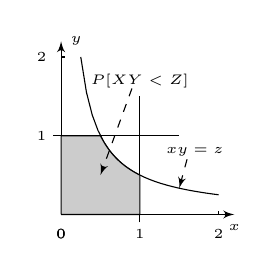
\begin{tikzpicture}[auto, >=latex']{scale = 2}
\draw[->](0,0)--(2.2,0)node[left,below,font=\tiny]{$x$};
\draw[->](0,0)--(0,2.2)node[right,font=\tiny]{$y$};
\draw(-0.1,1)--(1.5,1); % \draw[dashed](-0.1,1)--(1.5,1)
\draw(1,-0.1)--(1,1.5);
\foreach \x in {0,0,0,1,2}{\draw(\x,0)--(\x,0.05)node[below,outer sep=2pt,font=\tiny]at(\x,0){\x};}
\foreach \y in {1,2}{\draw(0,\y)--(0.05,\y)node[left,outer sep=2pt,font=\tiny]at(0,\y){\y};}
\draw[color=black ,domain=0.25:2]plot(\x,{0.5/(\x)});
\filldraw [fill=gray!40] (0,0) -- (0,1)--(0.5,1)--plot [domain=0.5:1,smooth] (\x,{0.5/(\x)})  -- (1,0.5)--(1,0)--(0,0);
\draw node at (1,1.7){\tiny $P[XY<Z]$};
\draw[->][dashed](0.9,1.6)--(0.5,0.5);
\draw node at (1.7,0.8){\tiny$xy=z$};
\draw[->][dashed](1.6,0.7)--(1.5,0.333);
\end{tikzpicture}
\end{center}
\[
\therefore F_{Z}(z)=\left\{\begin{array}{ll}{1} & {z \geq 1} \\ {0} & {z \leq 0} \\ {z+\int_{z}^{1} \int_{0}^{\frac{2}{x}} f_{X Y}(x, y) d y d x} & {0<z<1}\end{array}\right.
\]
Since $f_{X Y}(x, y)=1 \quad 0<x<1, \quad 0<y<1$,
\[
\begin{array}{rlrl}{\Rightarrow F_{Z}(z)} & {=z+\int_{z}^{1} \int_{0}^{\frac{2}{x}} d y d x=z+\int_{z}^{1} \frac{z}{x} d x} \\ {} & {=z-z \ln z} & {0<z<1} \\ {\Rightarrow f_{Z}(z)} & {=\frac{d F_{Z}(z)}{d z}=-\ln z} & {0<z<1}\end{array}
\]
 \section* {Problem 2} 
Determine the pdf of $Y, f_{Y}(y)$, where $Y=\sin X$, and $X$ is a uniform random variable with pdf

\[
f_{X}(x)=\left\{\begin{array}{cc}{\frac{1}{2 \pi}} & {-\pi<x \leq \pi} \\ {0} & {\text { otherwise }}\end{array}\right.
\]
\section* {Solution} 
PDF of random variable $Y$ is given by:
\[
F_{Y}(y)=P[Y \leq y]=\left\{\begin{array}{cl}{1} & {y \geq 1} \\ {0} & {y<-1} \\ {P[\sin X \leq y]} & {-1 \leq y<1}\end{array}\right.
\]
Then,
\[
\begin{aligned} P[\sin X \leq y] &=1-P[\sin X \geq y] \\ &=2 P[X \leq \arcsin y] \\ &=2 \int_{-\frac{\pi}{2}}^{\arcsin y} f_{X}(x) d x=2 \int_{-\frac{\pi}{2}}^{\arcsin y} \frac{1}{2 \pi} d x \\ &=\frac{1}{\pi}\left(\arcsin y+\frac{\pi}{2}\right) \end{aligned}
\]
Therefore,
\[
\therefore f_{Y}(y)=\frac{d F_{Y}(y)}{d y}=\frac{1}{\pi \sqrt{1-y^{2}}} \qquad-1 \leq y<1
\]
\section* {Problem 3} 
Let $X_{1}, X_{2},$ and $X_{3}$ be random variables with equal variances but with correlation coefficients $\rho_{12}=$
$0.3, \rho_{13}=0.5,$ and $\rho_{23}=0.2 .$ Find the correlation coefficient of the linear functions $Y=X_{1}+X_{2}$
and $Z=X_{2}+X_{3}$
\section* {Solution} 
Let $\sigma^{2}$ be the variance of $X_{1}, X_{2}, X_{3}$ . Then,
\[\left\{\begin{array}{l}{\operatorname{Cov}\left[X_{1}, X_{2}\right]=\sigma^{2} \rho_{12}} \\ {\operatorname{Cov}\left[X_{1}, X_{3}\right]=\sigma^{2} \rho_{13}} \\ {\operatorname{Cov}\left[X_{2}, X_{3}\right]=\sigma^{2} \rho_{23}}\end{array}\right.\]
Using this,
\[
\begin{aligned} \begin{split}\operatorname{Cov}[Y, Z] &=\mathbb{E}\left[\left(X_{1}+X_{2}\right)\left(X_{2}+X_{3}\right)\right]-\mathbb{E}\left[X_{1}+X_{2}\right] \mathbb{E}\left[X_{2}+X_{3}\right] \\ &=\mathbb{E}\left[X_{1} X_{2}\right]+\mathbb{E}\left[X_{1} X_{3}\right]+\mathbb{E}\left[X_{1}^{2}\right]+\mathbb{E}\left[X_{2}X_{3}\right]-\mathbb{E}\left[X_{1}\right]\mathbb{E}\left[X_{2}\right]\\&\quad-\mathbb{E}\left[X_{1}\right]\mathbb{E}\left[X_{3}\right]-\mathbb{E}\left[X_{1}\right]^{2}-\mathbb{E}\left[X_{2}\right] \mathbb{E}\left[X_{3}\right] \\ &=\operatorname{Cov}\left[X_{1}, X_{2}\right]+\operatorname{Cov}\left[X_{1}, X_{3}\right]+\sigma^{2}+\operatorname{Cov}\left[X_{2}, X_{3}\right] \\ &=\sigma^{2}\left(\rho_{12}+\rho_{13}+1+\rho_{23}\right)\end{split} \end{aligned}
\]
On the other hand, the variances of $Y$ and $Z$ are:
\[
\begin{aligned} \sigma_{Y}^{2} &=\mathbb{E}\left[\left(X_{1}+X_{2}\right)\left(X_{1}+X_{2}\right)\right]-\mathbb{E}\left[X_{1}+X_{2}\right] \mathbb{E}\left[X_{1}+X_{2}\right] \\ &=2 \sigma^{2}+2 \operatorname{Cov}\left[X_{1}, X_{2}\right]=2 \sigma^{2}\left(1+\rho_{12}\right) \\ \sigma_{Z}^{2} &=\mathbb{E}\left[\left(X_{2}+X_{3}\right)\left(X_{2}+X_{3}\right)\right]-\mathbb{E}\left[X_{2}+X_{3}\right] \mathbb{E}\left[X_{2}+X_{3}\right] \\ &=2 \sigma^{2}+2 \operatorname{Cov}\left[X_{2}, X_{3}\right]=2 \sigma^{2}\left(1+\rho_{23}\right) \\ \therefore \rho_{Y Z} &=\frac{\operatorname{Cov}[Y, Z]}{\sigma_{Y} \sigma_{Z}}=\frac{\rho_{12}+\rho_{13}+1+\rho_{23}}{\sqrt{2+2 \rho_{12}} \sqrt{2+\rho_{23}}}=\frac{2}{\sqrt{2.6} \sqrt{2.4}}=0.8006 \end{aligned}
\]
\section* {Problem 4} 
Let
\[
f\left(x_{1}, x_{2}\right)=\left\{\begin{array}{cc}{6 x_{1}} & {0<x_{1}<x_{2}<1} \\ {0} & {\text { elsewhere }}\end{array}\right.
\]
be the joint pdf of the random variables $X_{1}$ and $X_{2}$ .
\begin{enumerate}
\item Find the conditional mean and variance of $X_{1},$ given $X_{2}=x_{2}, 0<x_{2}<1$
\item Find the pdf of the random variable $Y=\mathbb{E}\left[X_{1} | X_{2}\right]$
\item Determine $\mathbb{E}[Y]$ and $\operatorname{Var}[Y]$ and compare these to $\mathbb{E}\left[X_{1}\right]$ and $\operatorname{Var}\left[X_{1}\right],$ respectively. What can
we know about the results?
\end{enumerate}
\section* {Solution} 
\begin{enumerate}
\item The marginal pdf of $X_{1}$ is:
\[
f_{2}\left(x_{2}\right)=\left\{\begin{array}{ll}{\int_{0}^{x_{2}} 6 x_{1} d x_{1}=3 x_{2}^{2}} & {0<x_{2}<1} \\ {0} & {\text { elsewhere }}\end{array}\right.
\]
Then, the conditional pdf of $X_{1},$ given $X_{2}=x_{2},$ is:
\[
f_{1 | 2}\left(x_{1} | x_{2}\right)=\left\{\begin{array}{cc}{\frac{f\left(x_{2}, x_{1}\right)}{f_{2}\left(x_{2}\right)}=\frac{6 x_{1}}{3 x_{2}^{2}}=\frac{2 x_{1}}{x_{2}^{2}}} & {0<x_{1}<x_{2}} \\ {0} & {\text { elsewhere }}\end{array}\right.
\]
Therefore,
\[
\therefore \mathbb{E}\left[X_{1} | x_{2}\right]=\int_{0}^{x_{1}} x_{2}\left(\frac{2 x_{1}}{x_{2}^{2}}\right) d x_{1}=\frac{2}{3} x_{2} \qquad 0<x_{2}<1
\]
\item From the above result, $Y=\mathbb{E}\left[X_{1} | X_{2}\right]=\frac{2 X_{2}}{3} .$ Then the PDF of $Y$ is:
\[
F_{Y}(y)=P[Y \leq y]=P\left[X_{2} \leq \frac{3 y}{2}\right] \qquad 0 \leq y<\frac{2}{3}
\]
Using the marginal pdf $f_{2}\left(x_{2}\right)$,
\[
F_{Y}(y)=\int_{0}^{\frac{3 y}{2}} 3 x_{2}^{2} d x_{1}=\frac{27 y^{3}}{8} \quad 0 \leq y<\frac{2}{3}
\]
\[
\therefore f_{Y}(y)=\frac{d F_{Y}(y)}{d y}=\frac{81 y^{2}}{8} \quad 0 \leq y<\frac{2}{3}
\]
\item Using the pdf $f_Y(y)$,
\[
\mathbb{E}[Y]=\int_{0}^{\frac{2}{3}} y \frac{81 y^{2}}{8} d y=\frac{1}{2}
\]
\[
\operatorname{Var}[Y]=\int_{0}^{\frac{2}{3}} y^{2} \frac{81 y^{2}}{8} d y-\left(\frac{1}{2}\right)^{2}=\frac{1}{60}
\]
On the other hand, the marginal pdf of $X_{1}$ is:
\[
f_{1}\left(x_{1}\right)=\int_{x_{1}}^{1} 6 x_{1} d x_{2}=6 x_{1}\left(1-x_{1}\right) \qquad 0<x_{1}<1
\]
zero elsewhere. Thus, it is easy to show that $\mathbb{E}\left[X_{1}\right]=\frac{1}{2}$ and $\operatorname{Var}\left[X_{1}\right]=\frac{1}{20} .$ That is, here
\[
\mathbb{E}[Y]=\mathbb{E}\left[\mathbb{E}\left[X_{1} | X_{2}\right]\right]=\mathbb{E}\left[X_{1}\right]
\]
and
\[
\operatorname{Var}[Y]=\operatorname{Var}\left[\mathbb{E}\left[X_{1} | X_{2}\right]\right] \leq \operatorname{Var}\left[X_{1}\right]
\]
$\Rightarrow$ This result has the useful interpretation. Both the random variables $X_{1}$ and $\mathbb{E}\left[X_{1} | X_{2}\right]$ have the same mean. If we did not know the mean, we could use either of the two random variables to guess at the mean. Since, however, Var $\left[\mathbb{E}\left[X_{1} | X_{2}\right]\right) \leq \operatorname{Var}\left[X_{1}\right],$ we would put more reliance in $\mathbb{E}\left[X_{1} | X_{2}\right]$ as a guess. That is we observe $x_{2}$, we could prefer to use $\mathbb{E}\left[X_{1} | x_{2}\right]$ as a guess at the unknown mean of $X_{1}$. Indeed, the general estimation approaches based on the incoming measurements are motivated by this idea.
\end{enumerate}
\section* {Problem 5} 
Consider a Gaussian random vector $X=\left[X_{1}, X_{2}\right]^{T}$ with expectation and covariance matrix given by:
\[
E(x)=\left[\begin{array}{l}{0} \\ {0}\end{array}\right], K :=\operatorname{Cov}(X)=\left[\begin{array}{ll}{2} & {1} \\ {1} & {4}\end{array}\right]
\]
\begin{enumerate}
\item Find the eigenvalues and eigenvectors of $K$
\item The contours of equal probability density (likelihood ellipse) are given by an equation of the
	form
	\[
	x^{T} K^{-1} x=c^{2}
	\]
\item Plot the likelihood ellipses for $c=0.25,1,1.5$
\item What is the probability of finding $x$ inside each of these ellipses?
\end{enumerate}
\section*{Solution}
\begin{enumerate}
\item Eigenvalues $\lambda$ are given by
\[
\operatorname{det}(\lambda I-K)=\lambda^{2}-6 \lambda+7=0
\]
\[
\therefore \lambda_{1}=1.5858, \lambda_{2}=4.4141
\]
and the corresponding eigenvectors are
\[
\operatorname{det}\left(\lambda_{1} I-K\right) v_{1}=0 \rightarrow v_{1}=[-0.9239 \quad 0.3827]^{\mathrm{T}}
\]
\[
\operatorname{det}\left(\lambda_{2} I-K\right) v_{2}=0 \rightarrow v_{2}=[-0.3827 \quad 0.9239]^{\mathrm{T}}
\]
\item Let $Q=\left[v_{1} v_{2}\right]$ and $x :=Q y .$ Then, since,
\[
Q^{\mathrm{T}} K Q=\Lambda=\left[\begin{array}{cc}{\lambda_{1}} & {0} \\ {0} & {\lambda_{2}}\end{array}\right] \rightarrow Q^{\mathrm{T}} K^{-1} Q=\Lambda^{-1}
\]
we have
\[
x^{\mathrm{T}} K^{-1} x=y^{\mathrm{T}} \Lambda^{-1} y=\sum_{i=1}^{2} \frac{y_{i}^{2}}{\lambda_{i}}=c^{2}
\]
which is an ellipse equation. Thus, the directions of eigenvectors are principal axes. Specifically,
$v_{2}$ is major axis and $v_{1}$ in minor axis.
\item The distances from the origin to the ellipsoid in the principal axes directions are $c \sqrt{\lambda_{2}}$ and $c \sqrt{\lambda_{1}}$ . Therefore, the ellipses for different $c$ are given by
\item The probability of finding $x$ inside each of these ellipses is given by:
\[
P\left[x^{T} K^{-1} x \leq c^{2}\right]=P\left[y^{T} \Lambda^{-1} y \leq c^{2}\right]=1-\exp \left(-\frac{c^{2}}{2}\right)
\]
and thus for the differnt $c$ cases,
\[
\left\{\begin{array}{l}{c=0.25 \rightarrow P=3.08 \%} \\ {c=1 \rightarrow P=39.35 \%} \\ {c=1.5 \rightarrow P=67.53 \%}\end{array}\right.
\]
\end{enumerate}
\section* {Problem 6} 
Given the three estimates of the scalar $x$
\[
y_{i} :=\hat{x}_{i}=x+\tilde{x}_{i}, \quad i=1,2,3
\]
with the estimation error $\tilde{x}_{i}$ jointly Gaussian, zero-mean, with
\[
E\left[\tilde{x}_{i} \tilde{x}_{i}\right]=P_{i j}, \quad i, j=1,2,3
\]
Find
\begin{enumerate}
\item The maximum likelihood estimator
\item The variance of the maximum likelihood estimator
\end{enumerate}
\section*{Solution}
\begin{enumerate}
\item The maximum likelihood estimator of $x$ given $y_{i}, i=1,2,3$ is represented as
\[
\begin{aligned} \hat{x}_{M L} &=\arg \max _{x} P\left[y_{1}, y_{2}, y_{3} | x\right] \\ &=\arg \max _{x} \Lambda_{Y}(x) \end{aligned}
\]
where
\[
\Lambda_{Y}(x)=\frac{1}{2 \pi^{\frac{3}{2}} \sqrt{|P|}} \exp \left(-\frac{1}{2}\left[y_{1}-x \quad y_{2}-x y_{3}-x\right] P^{-1}\left[y_{1}-x \quad y_{2}-x \quad y_{3}-x\right]^{\mathrm{T}}\right)
\]
\[
P=\left[\begin{array}{lll}{P_{11}} & {P_{12}} & {P_{13}} \\ {P_{21}} & {P_{22}} & {P_{23}} \\ {P_{31}} & {P_{32}} & {P_{33}}\end{array}\right]
\]
Then, it is equivalnet that
\[
\max \Lambda_{Y}(x)=\min \left[y_{1}-x \quad y_{2}-x y_{3}-x\right] P^{-1}\left[y_{1}-x \quad y_{2}-x \quad y_{3}-x\right]^{\mathrm{T}}
\]
Therefore, the given ML estimator can be interpreted as the least-square (LS) estimator as
follows
\[
\hat{x}_{M L}=\hat{x}_{L S}=\left(H^{\mathrm{TP}-1} H\right)^{-1} H^{\mathrm{T}} P^{-1}\left[\begin{array}{c}{y_{1}} \\ {y_{2}} \\ {y_{3}}\end{array}\right]
\]
where $H=\left[\begin{array}{lll}{1} & {1} & {1}\end{array}\right]^{\mathrm{T}}$.
\item The estimation error of the ML estimator, $e :=\hat{x}_{M L}-x,$ is given by
\[
e=\left(H^{\mathrm{T}} P^{-1} H\right)^{-1} H^{\mathrm{T}} P^{-1}\left[\begin{array}{c}{\tilde{x}_{1}} \\ {\tilde{x}_{2}} \\ {\tilde{x}_{3}}\end{array}\right]
\]
Since $\mathbb{E}[e]=0$,
\[
\begin{aligned} \operatorname{Var}(e)=\mathbb{E}\left[e^{2}\right] &=\mathbb{E}\left[\left(H^{\mathrm{T}} P^{-1} H\right)^{-1} H^{\mathrm{T}} P^{-1}\left[\begin{array}{c}{\tilde{x}_{1}} \\ {\tilde{x}_{2}} \\ {\tilde{x}_{3}}\end{array}\right]\right.\\=&\left(H^{\mathrm{T}} P^{-1} H\right)^{-1} H^{\mathrm{T}} P^{-1} \mathbb{E}\left[\left[\begin{array}{c}{\tilde{x}_{1}} \\ {\tilde{x}_{2}} \\ {\tilde{x}_{2}}\end{array}\right]\left[\begin{array}{ccc}{\tilde{x}_{1}} & {\tilde{x}_{2}} & {\tilde{x}_{3} ]}\end{array}\right] P^{-1} H\left(H^{\mathrm{T}} P^{-1} H\right)^{-1}\right] \\ &=\left(H^{\mathrm{T}} P^{-1} H\right)^{-1} H^{\mathrm{T}} P^{-1} P P^{-1} H\left(H^{\mathrm{T}} P^{-1} H\right)^{-1} \\ &=\left(H^{\mathrm{T}} P^{-1} H\right)^{-1} \end{aligned}
\]
\end{enumerate}
\section* {Problem 7} 
Consider a random vector $Y=[y(1) y(2) \cdots y(k)]^{\mathrm{T}}$ where the elements $y(j)$ are made
\[
y(j)=x+w(j), \quad j=1, \cdots, k
\]
where $w(j)$ are independent, identically distributed, Gaussian, zero-mean, and with the variance $\sigma^{2}$ ,
i.e., $\mathcal{N}\left(0, \sigma^{2}\right) .$
\begin{enumerate}
	\item Find the Maximum Likelihood (ML) estimator for $x,$ i.e., $\hat{x}_{M L}$
	\item Find the Mean Square Error (MSE) of ML estimator, i.e., $\operatorname{MSE}\left(\hat{\mathbf{x}}_{M L}\right) \equiv \operatorname{Var}\left(\hat{x}_{M L}\right)$
	\item Is this estimator consistent? Prove your answer
	\item Is this estimator efficient? Prove your answer
\end{enumerate}
\section*{Solution}
\begin{enumerate}
\item The ML estimator is given by
\[
\hat{x}_{M L}=\arg \max _{x} P(Y | x)=\arg \max _{x} \Lambda_{Y}(x)
\]
where the likelihood function $\Lambda_{Y}(x)$ is
\[
\Lambda_{Y}(x)=\frac{1}{2 \pi^{k / 2} \sqrt{|\Sigma|}} \exp \left\{-\frac{1}{2}[Y-\overline{1} x]^{\mathrm{T}} \Sigma^{-1}[Y-\overline{1} x]\right\}
\]
where $\Sigma \in \mathbb{R}^{k \times k}$ and $\overline{1} \in \mathbb{R}^{k}$ are respectively given as
\[
\Sigma=\left[\begin{array}{cccc}{\sigma^{2}} & {0} & {\cdots} & {0} \\ {0} & {\sigma^{2}} & {\cdots} & {0} \\ {\vdots} & {\vdots} & {\ddots} & {\vdots} \\ {0} & {\cdots} & {\cdots} & {\sigma^{2}}\end{array}\right]=\sigma^{2} I, \quad \overline{1}=\left[\begin{array}{c}{1} \\ {1} \\ {\vdots} \\ {1}\end{array}\right]
\]
Then,
\[
\begin{aligned} \arg \max _{x} \Lambda_{Y}(x) &=\arg \min _{x}\left(\frac{1}{2}[Y-\overline{1} x]^{\mathrm{T}} \Sigma^{-1}[Y-\overline{1} x]\right) \\ &=\arg \min _{x}\left(\frac{1}{2 \sigma^{2}}[Y-\overline{1} x]^{\mathrm{T}}[Y-\overline{1} x]\right) \end{aligned}
\]
From the right-hand-side term of the above equation, ML estimator can be interpreted as the
exactly same formulation as the Least Square (LS) estimator whose minimum solution is
\[
\hat{x}_{M L}=\hat{x}_{L S}=\left(\overline{1}^{\mathrm{T}} \overline{1}\right)^{-1} \overline{1}^{\mathrm{T}} Y=\frac{1}{k} \sum_{j=1}^{k} y(j)
\]
\item MSE of the $\hat{x}_{M L}$ is defined as MSE $\left(\hat{\mathrm{x}}_{\mathrm{ML}}\right) :=\mathbb{E}\left[\left(\hat{x}_{M L}-x\right)^{2}\right] .$ From the previous result,
\[\begin{aligned} \mathbb{E}\left[\left(\hat{x}_{M L}-x\right)^{2}\right] &=\mathbb{E}\left[\left(\frac{1}{k} \sum_{j=1}^{k} y(j)-x\right)^{2}\right] \\ &=\mathbb{E}\left[\left(\frac{1}{k} \sum_{j=1}^{k}(x+w(j))-x\right)^{2}\right]=\mathbb{E}\left[\left(\frac{1}{k} \sum_{j=1}^{k} w(j)\right)^{2}\right]\\&=\frac{\sigma^{2}}{k} \end{aligned}\]
\item Check the consistency:
\[
\lim _{k \rightarrow \infty} \operatorname{MSE}\left(\hat{\mathrm{x}}_{\mathrm{ML}}\right)=\lim _{k \rightarrow \infty} \frac{\sigma^{2}}{k}=0
\]
$\therefore$ The given ML estimator is consistent so that the solution is getting more accurate as we
take more measurements.
\item Check the efficiency: Cramer-Rao Lower Bound (CRLB) for the MSE of the given ML estimator
is
\[
\operatorname{MSE}\left(\hat{\mathbf{x}}_{M L}\right) \geq J^{-1}
\]
where
\[
\begin{aligned} J & :=\mathbb{E}\left[\left(\frac{\partial \ln \Lambda_{Y}(x)}{\partial x}\right)^{2}\right]=\mathbb{E}\left[\left(-\frac{1}{2 \sigma^{2}} \frac{\partial[Y-\overline{1} x]^{\mathrm{T}}[Y-\overline{1} x]}{\partial x}\right)^{2}\right] \\ &=\mathbb{E}\left[\left(\frac{2 \overline{1}^{\mathrm{T}} \overline{1} x-2 \overline{1}^{\mathrm{T}} Y}{2 \sigma^{2}}\right)^{2}\right]=\mathbb{E}\left[\left(\frac{2 \overline{1}^{\mathrm{T}} \overline{1} x-2 \overline{1}^{\mathrm{T}} \overline{1} x-2 \sum_{j=1}^{k} w(j)}{2 \sigma^{2}}\right)^{2}\right] \\ &=\mathbb{E}\left[\left(\frac{-\sum_{j=1}^{k} w(j)}{\sigma^{2}}\right)^{2}\right]=\frac{k \sigma^{2}}{\sigma^{4}}=\frac{k}{\sigma^{2}} \end{aligned}
\]
Therefore,
\[
\operatorname{MSE}\left(\hat{\mathrm{x}}_{\mathrm{ML}}\right)=\frac{\sigma^{2}}{k}=J^{-1}
\]
$\therefore$ Since the estimator's MSE(variance) is equal to its CRLB, the given ML estimator is efficient.
\end{enumerate}
\end{document}